% !TEX encoding = UTF-8
% !TEX TS-program = pdflatex
% !TEX root = ../tesi.tex

%**************************************************************
\chapter{Progettazione}
\label{cap:progettazione}
%**************************************************************
\section{Studio AR Anchor}
\label{sec:ar-anchor}
\subsection{Azure Spatial Anchors}
\label{subsec:asa}
\subsection{Google Cloud Anchors}
\label{subsec:gca}

%**************************************************************
\section{Confronto framework AR}
\label{sec:confronto-framework}
Essendo lo scopo di questo stage, e quindi il caso di studio di questa tesi, l'implementazione di una vista in realtà aumentata (nello specifico sfruttando asa) in un'applicazione preesistente sviluppata in Flutter, una grossa parte del lavoro svolto si è incentrato sullo studio dei framework e/o plug-in disponibili.\\
Sfortunatamente, complici la giovinezza di Flutter e la scarsa diffusione di tecnologie AR, le opzioni disponibili sono alquanto ridotte:
\begin{itemize}
    \item \textit{ar\_flutter\_plugin}: \href{https://pub.dev/packages/ar_flutter_plugin}{plugin} che punta a implementare le componenti AR in modalità cross-platform, quindi adattandosi autonomamente ad Android e iOS (sfruttando tuttavia le Cloud Anchor di Google). Nasce partendo da due plugin più specializzati: 
    \begin{itemize}
        \item \textit{arcore\_flutter\_plugin} (\href{https://github.com/giandifra/arcore_flutter_plugin}{Android});
        \item \textit{arkit\_flutter\_plugin} (\href{https://github.com/olexale/arkit_flutter_plugin}{iOS});
    \end{itemize}
    \item \textit{ARwayKit}: framework che mira a fornire un'integrazione semplificata, e in parte già completata, di una componente AR (ottenuta tramite asa) in Flutter tramite vista in Unity.
\end{itemize}
{\footnotesize Al momento della stesura di questo testo non è più possibile accedere liberamente alla \href{https://app.gitbook.com/s/-MCtct_TY9f3e8PrcV9T/arwaykit-with-flutter/quickstart-in-flutter}{documentazione} relativa ad ARwayKit, tuttavia è ancora reperibile un \href{https://medium.com/arway/building-ar-navigation-apps-with-flutter-and-arwaykit-280b69401cd9}{articolo} su \textit{medium.com} che ricalca la guida introduttiva precedentemente fornita dal sito ufficiale dell'azienda (è anche possibile trovarne una \href{https://web.archive.org/web/20220525060655/https://docs.arway.app/arwaykit-with-flutter/quickstart-in-flutter}{versione nella Wayback Machine}).}

\subsection{ARwayKit}
\label{subsec:arwaykit}
ARwayKit è un framework formato da un insieme di componenti che si pone l'obiettivo di fornire un'esperienza AR persistente, e lo persegue fornendo una SDK Unity, un'applicazione di Mapping e un insieme di API REST, che implementa le componenti AR in Flutter sfruttando \href{https://pub.dev/packages/flutter_unity_widget}{flutter\_unity\_widget}.\\
\E{} cross-platform, implementa le Anchor tramite asa e funziona in ambienti "gps-denied", ovvero dove i dati di posizone del gps non vengono utilizzati per muoversi all'interno dell'ambiente virtuale (oppure ambienti con protocolli di privacy elevati), il che lo rende apparentemente perfetto per il caso d'uso specifico di questa tesi, tuttavia presenta delle criticità: in primo luogo obbliga l'uso di Unity (sfruttando la sua caratteristica peculiare di poter essere importato come fosse una libreria) per sviluppare la vista AR, il che comporta non solo dover imparare il linguaggio ma dover anche configurare ulteriori componenti (come ad esempio \textit{Unity Hub}) che poi devono essere adottati assieme a quelli già in uso, appesantendo quindi il processo di codifica.\\
In secondo luogo troviamo invece il problema maggiore: la vista verrebbe realizzata nativamente in Unity, ovvero si tratta di una componente Unity separata rispetto all'applicazione che la lancia.
Questo renderebbe complesso se non impossibile usare dentro essa delle funzionalità Flutter: ad esempio, un bottone a schermo sarebbe un pulsante Unity, non Flutter, obbligando quindi poi a costruire una mappatura tra i due linguaggi per ogni funzionalità visualizzata.\\ 
Una vista così costruita non solo è scomoda da programmare, ma anche difficile da manutenere.\\

\begin{figure}[h!]
    \centering
    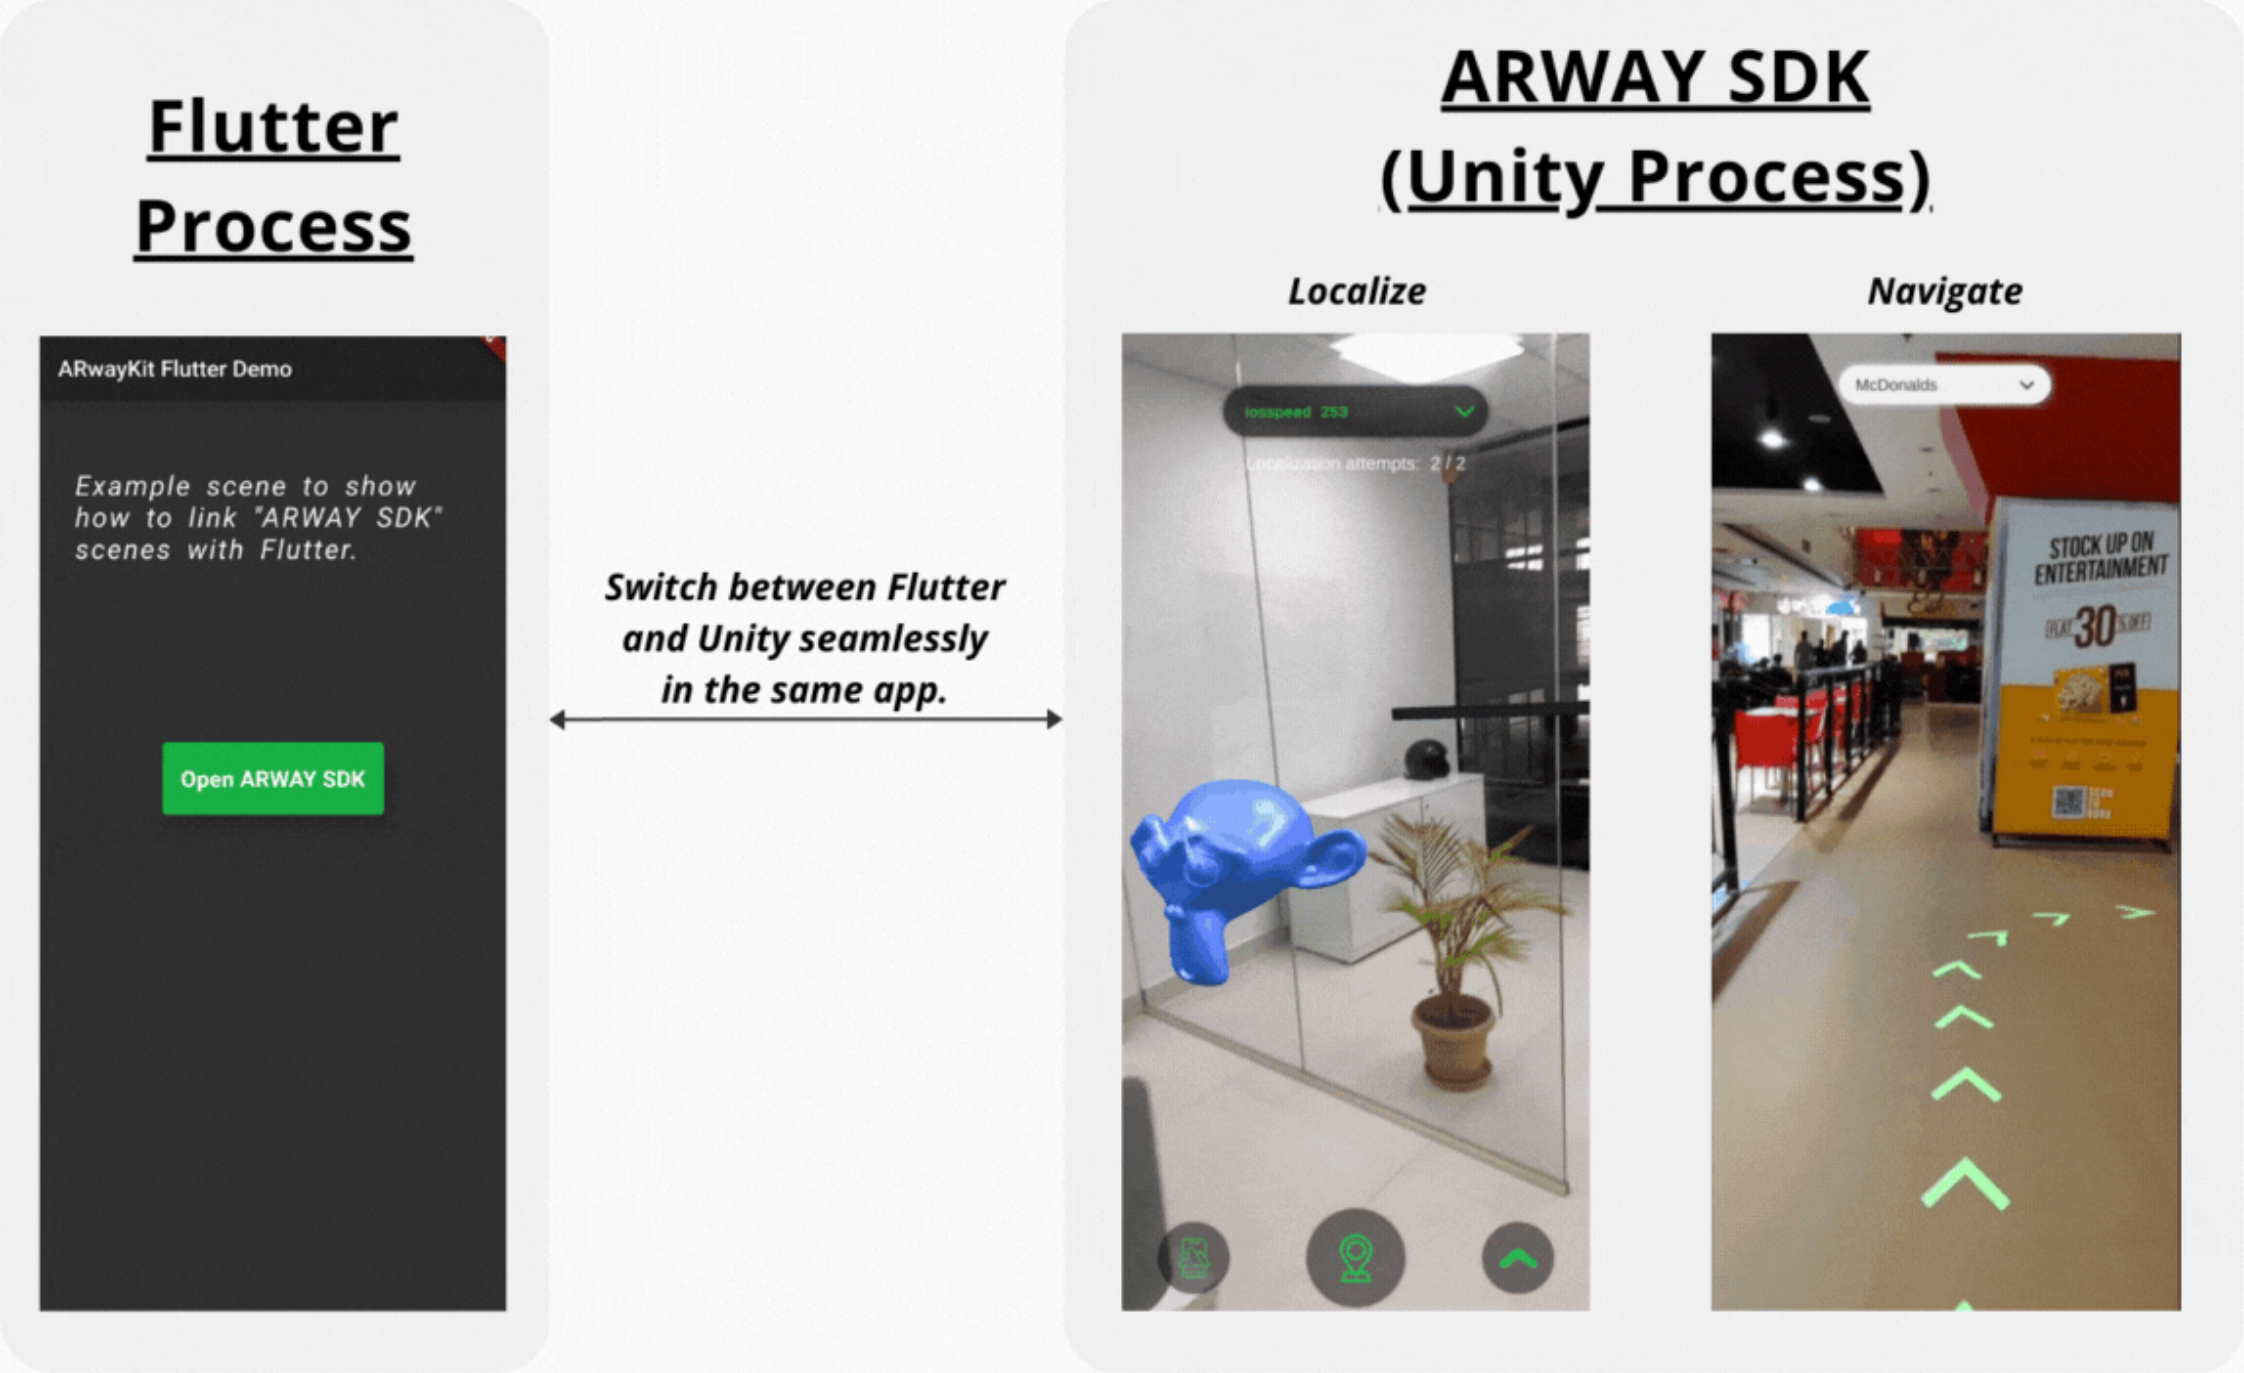
\includegraphics[height=5cm]{ARwayKit_samplegif_screenshot}
    \caption{Immagine esempio di utilizzo AR con ARwayKit}
\end{figure}


\subsection{ar\_flutter\_plugin}
\label{subsec:ar_flutter_plugin}
\arplug{} è un plugin open source collaborativo estremamente giovane (il primo commit sulla repository pubblica risale al 6 febbraio 2021) che si pone l'obiettivo di implementare componenti in realtà aumentata in Flutter.\\
Per raggiungere lo scopo si serve della libreria archiviata \href{https://developers.google.com/sceneform/develop}{Sceneform}, che si occupa di "renderizzare scene 3D realistiche in applicazioni AR o meno, senza dover imparare OpenGL".\\
L'architettura di \arplug{} è composta da due parti: una API cross-platform unificata che fornisce un'interfaccia alle applicazioni tramite il plugin e le implementazioni specifiche per le piattaforme Android (in Kotlin) e iOS (in Swift) costruite su ARCore e ARKit rispettivamente, così da garantire accesso continuativo nel tempo a funzionalità aggiornate.\\
\arplug{} espone dei widget e delle classi 



\subsubsection{il nostro ar flut plug}
fork per asa 
"com.gorisse.thomas.sceneform:sceneform:1.21.0" 

%----------------------------------------------------------------
\section{integrazione asa ar flut plug}
\label{sec:progettazione-onboarding-primo-login}


%----------------------------------------------------------------
\subsection{flutter <-> ar flut plug}
\label{sec:autenticazione-tramite-auth0}
passaggio dati app mobilesyn con ar flut plug (assets etc)

[diagramma comunicazione plug in ar - flutter]


\subsection{Chiamate asincrone}
Un punto chiave per lo sviluppo dell'app è quello delle chiamate asincrone.\\
Quando una funzione richiede molto tempo per essere completata, come ad esempio una funzione che richiede dati ad un un server, è opportuno chiamarla in modo asincrono, così da non fermare tutta l'applicazione in attesa del completamento di quella funzione. Utilizzando le chiamate asincrone infatti il flusso delle operazioni che non necessitano il termine della chiamata può continuare indisturbato.\\
Dart mette a disposizione due modi per la gestione di questo tipo di chiamate, noi in accordo comune abbiamo deciso di usare il metodo \textit{async} e \textit{await}: le funzioni che prevedono la possibilità di fare chiamate asincrone sono contrassegnate con la parola chiave \textit{async}. All'interno delle funzioni asincrone è possibile quindi usare la parola chiave \textit{await} che serve per dire al programma di attendere quell'istruzione prima di proseguire con la successiva. Se non viene utilizzato il comando \textit{await} allora tale funzione asincrona verrà eseguita parallelamente al proseguo del programma fino al suo completamento.\\
\begin{figure}[h!]
    \centering
    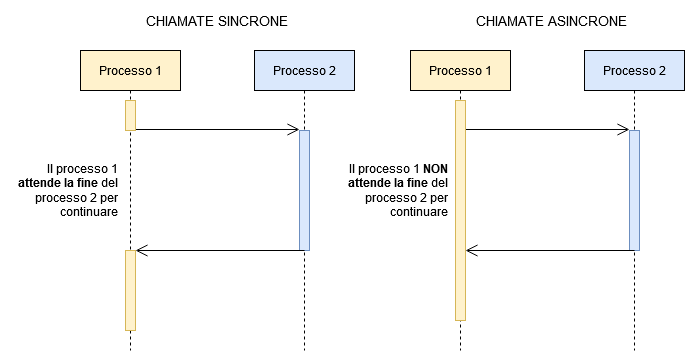
\includegraphics[height=6cm]{async}
    \caption{Chiamate sincrone VS asincrone}
\end{figure}
%*********************************************************************
\subsection{progettazione UI ux}

Essendo l'applicazione un supporto ad una piattaforma di analisi dati la presenza di chiamate asincrone al backend è molto frequente, è stato quindi fondamentale progettare un pattern solido da riutilizzare per ogni chiamata.
Il \textit{pattern} da noi adottato prevede che una qualsiasi chiamata API CRUD possa trovarsi in tre diversi stati:
\begin{itemize}
    \item \textbf{Loading}: la chiamata è iniziata e non è ancora stata risolta;
    \item \textbf{Error}: la chiamata è terminata con un errore;
    \item \textbf{Response}: la chiamata è terminata e possiedo i dati di mio interesse.
\end{itemize}
Appena prima di inviare la richiesta HTTP l'applicazione viene messa in uno stato di \textit{loading}, nel caso di errori al backend o nessuna risposta ci si troverà in uno stato di \textit{error}, altrimenti, nel caso in cui il backend risponda con i dati corretti ci si troverà in uno stato di \textit{response}.\\
L'interfaccia dunque cambierà in base allo stato della chiamata, mostrando un indicatore di progresso mentre ci si trova in uno stato di \textit{loading}, mostrando un errore nel caso ci si trovasse in uno stato di \textit{error}, o mostrando i dati elaborati nel caso di \textit{response}.
\begin{figure}[h!]
    \centering
    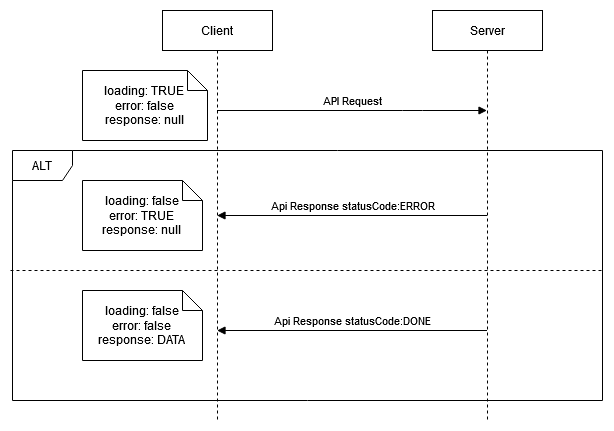
\includegraphics[height=8cm]{api}
    \caption{Diagramma di sequenza di una richiesta API}
\end{figure}
\begin{lstlisting}[language=dart, firstnumber=1,caption={User provider}]
final userChangeNotifier =
    ChangeNotifierProvider<UserRepo>((ref) => UserRepo(ref.read));
///Fornisce lo stato di errore di [UserRepo].
final userError = Provider((ref) => ref.watch(userChangeNotifier).error);
///Fornisce il messaggio di errore di [UserRepo].
final userErrorMsg = Provider((ref) => ref.watch(userChangeNotifier).errorMsg);
///Fornisce lo stato di loading di [UserRepo].
final userIsLoading =
    Provider((ref) => ref.watch(userChangeNotifier).isLoading);
///Fornisce l'istanza di [User].
final userProvider = Provider((ref) => ref.watch(userChangeNotifier).user);

class UserRepo extends ChangeNotifier {
  bool error = false;
  bool isLoading = false;
  String errorMsg = "";
  final String apiUrl = dotenv.env['API_URL'] ?? "";
  User? user;
  final Reader read;
  UserRepo(this.read);
  Future<void> fetchUser() async {
    var token = await read(authProvider).getAccessToken();
    this.isLoading=true;
	notifyListeners();
    try {
      final response = await Dio().get(
        apiUrl + "/api/myself",
        options: Options(
            headers: 
                <String, String>{'Authorization': 'Bearer $token'}),);
      if (response.statusCode == 200) {
        this.user = User.fromJson(response.data));
        this.isLoading = false;
      } else {
        this.isLoading = false;
        this.error = value;
        this.errorMsg = "richiesta fallita";
      }
    } catch (e) {
      this.isLoading = false;
	  this.error = value;
      this.errorMsg = "richiesta fallita";
    } finally {
	  notifyListeners();
    }
  }
}
\end{lstlisting}
%*************************************************************
\subsection{API di LifestyleSync}
Di seguito sono riportate alcune delle API utilizzate durante lo sviluppo delle applicazioni.\\
Esse si rifanno ad un modello REST-like e non REST puro in quanto tutte le richieste HTTP vengono firmate mediante la tecnica \gls{JWT} presentata in precedenza.\\
Le API verranno riportate nella forma [metodo\textunderscore HTTP][url/api]
\begin{enumerate}
    \item \textbf{GET api/myself}\\
    Restituisce un file JSON che descrive l'utente, con le sue info e i dettagli del suo coach, con il seguente schema:
    \begin{lstlisting}[language=json,firstnumber=1,caption={JSON schema dell'API GET api/myself},captionpos=b]
    {
    "user_id": String,
    "given_name": String,
    "family_name": String,
    "email": String,
    "picture": String,
    "info":
        {
        survey_done: bool,
        coach: Map<String, dynamic>,
        oms_thresh: Map<String, int>,
        fit_profiles: Map<String, dynamic>
        }
    "user_metadata": Map<String, dynamic>
    }
    \end{lstlisting}
    dove: \begin{itemize}
        \item user\textunderscore id: è l'identificativo dell'utente nel database;
        \item given\textunderscore name: è il nome dell'utente;
        \item family\textunderscore name: è il cognome dell'utente;
        \item email: è la e-mail dell'utente;
        \item picture: è il link dell'immagine del profilo dell'utente;
        \item user\textunderscore metadata: sono i meta-dati dell'utente;
        \item info:
        \begin{itemize}
            \item survey\textunderscore done: è true se l'utente ha completato il questionario;
            \item coach: sono i dati del coach dell'utente;
            \item oms\textunderscore thresh: sono le soglie da raggiungere secondo l'OMS;
            \item fit\textunderscore profiles: sono i profili fit dell'utente;
        \end{itemize}
    \end{itemize}
    \item \textbf{GET api/goals}\\
    Questa API accetta diversi parametri obbligatori:
    \begin{itemize}
        \item end: data di fine dei goals che voglio in formato \textit{IsoTime};
        \item active: se voglio i goals attivi o meno in formato \textit{Bool};
        \item interval: intervallo di tempo antecedente a \textit{end}, può essere: week, month, 3month o 6month in formato \textit{String}.
    \end{itemize}
    Restituisce un array di oggetti JSON che descrivono i goals dell'utente, con il seguente schema:
    \begin{lstlisting}[language=json,firstnumber=1,caption={JSON schema dell'API GET api/goals},captionpos=b]
    {
    "id": String,
    "u_id": String,
    "goals":
        {
        "calories":
            {
            "m": String,
            "thresh": int,
            }    
        "duration_activities":
            {
            "m": String,
            "thresh": int,
            }    
        "duration_normal":
            {
            "m": String,
            "thresh": int,
            }    
        "steps":
            {
            "m": String,
            "thresh": int,
            }    
        }
    "status":
        {
        "calories": int,
        "duration_activities": int,
        "duration_normal": int,
        "steps": int,
        }
    "start": IsoTime,
    "end": IsoTime,
    "achieved": bool,
    "active": bool,
    }
    \end{lstlisting}
    dove: \begin{itemize}
        \item id: è l'identificativo dell'obiettivo nel database;
        \item u\textunderscore id: è l'identificativo dell'utente nel database;
        \item goals:
        \begin{itemize}
            \item calories: sono le calorie da bruciare, \textit{m} è il tipo di metrica e \textit{thresh} è la soglia;
            \item duration\textunderscore activities: sono i minuti di attività da raggiungere, \textit{m} è il tipo di metrica e \textit{thresh} è la soglia;
            \item duration\textunderscore normal: sono i minuti attivi normali da raggiungere, \textit{m} è il tipo di metrica e \textit{thresh} è la soglia;
            \item steps: sono i passi da fare, \textit{m} è il tipo di metrica e \textit{thresh} è la soglia;
        \end{itemize}
        \item status:
        \begin{itemize}
            \item calories: sono le calorie bruciate;
            \item duration\textunderscore activities: sono i minuti di attività raggiunti;
            \item duration\textunderscore normal: sono i minuti attivi normali raggiunti;
            \item steps: sono i passi fatti;
        \end{itemize}
        \item start: è la data di inizio dell'obiettivo;
        \item end: è la data di fine dell'obiettivo;
        \item achieved: indica se l'obiettivo è stato raggiunto;
        \item active: indica se l'obiettivo è attivo.
    \end{itemize}
    \item \textbf{GET api/agendas}\\
    Questa API accetta diversi parametri obbligatori:
    \begin{itemize}
        \item end: data di fine degli appuntamenti che voglio in formato \textit{IsoTime};
        \item interval: intervallo di tempo antecedente a \textit{end}, può essere: week, month, 3month o 6month in formato \textit{String}.
    \end{itemize}
    Restituisce un array di oggetti JSON che descrivono gli appuntamenti, con il seguente schema:
    \begin{lstlisting}[language=json,firstnumber=1,caption={JSON schema dell'API GET api/agendas},captionpos=b]
    {
    "id": String,
    "start": IsoTime,
    "end": IsoTime,
    "subject": String,
    "tid": String,
    "notes": String,
    "coach": Map<String, dynamic>,
    "client": Map<String, dynamic>,
    }
    \end{lstlisting}
    dove: \begin{itemize}
        \item id: è l'identificativo dell'appuntamento nel database;
        \item start: è la data e ora di inizio dell'appuntamento;
        \item end: è la data e ora di fine dell'appuntamento;
        \item subject: è il titolo dell'appuntamento;
        \item notes: sono le note dell'appuntamento;
        \item tid: è il tenant a cui appartiene l'appuntamento;
        \item coach: sono i dettagli del coach;
        \item client: sono i dettagli del cliente.
    \end{itemize}
\end{enumerate}
%************************************************************
\subsection{Stato globale e locale}
Una delle problematiche principali quando si deve sviluppare un applicazione mobile o web è il come salvare i dati e gestire lo stato dell'applicazione.\\

Flutter prevede l’esistenza di due tipi di stato (simili ad uno \textit{store}): lo stato globale dell’applicazione, che ad ogni update causa un update dell’intero albero di \textit{rendering} dell’applicazione e lo stato locale, proprio del singolo widget e il cui update causa l’aggiornamento unicamente del widget stesso e dei suoi eventuali figli.\\
A seguito dell’analisi dei requisiti e del comportamento dell’applicazione si è deciso di utilizzare lo stato globale per i dati utilizzati da più widget con o senza legami di parentela. Mentre, seguendo il pattern \gls{SRP}, lo stato locale viene utilizzato dai widget che non condividono dati con altri componenti (ad esempio widget di pura presentazione o che rappresentano dati provenienti da un’API non sfruttata dall’intero applicativo).\\

Per la gestione dello stato globale abbiamo usato il provider pattern. Questo prevede l'utilizzo di un oggetto contenente i dati dell'applicazione che notifica ogni cambio di stato, il quale viene fornito all'applicazione utilizzando un \textit{provider}. In questo modo l'interfaccia grafica sarà sempre aggiornata con il valore corrente dello stato.\\
Per la gestione dello store globale si è deciso di utilizzare la libreria \textit{Riverpod}, questa fornisce una vasta scelta di \textit{provider} diversi, e rende più facile l'accesso ai dati grazie ad un hook da loro predisposto: \textit{useProvider}.
Per lo store locale invece, in seguito alla scelta di usare Flutter Hooks, abbiamo sfruttato l'hook \textit{useState}, questo costruisce una variabile che viene osservata dal componente, ad ogni cambiamento di questa variabile il componente si ricostruisce, aggiornandosi con il valore corrente dello stato.
%**************************************************************
\subsection{Routing iniziale}
Per questa prima parte del progetto è stato fondamentale progettare un buon routing per gestire correttamente i diversi casi di accesso.\\
Si è deciso per provare automaticamente il login all'avvio dell'applicazione utilizzando un token salvato nel \textit{secure storage} dello smartphone. Nel caso di accesso avvenuto con successo si prosegue, altrimenti si rimanda l'utente ad una schermata di login.\\
A questo punto è necessario controllare se è la prima volta che il cliente accede all'applicazione o meno, per fare questo controllo vengono richieste al \textbf{backend} le informazioni dell'utente e nel mentre viene mostrata una schermata di caricamento, a questo punto le possibili alternative di routing sono:
\begin{itemize}
    \item \textbf{Primo accesso}: viene mostrata all'utente una breve introduzione all'applicazione, gli viene presentato il suo coach, gli viene fatto rispondere ad un questionario rispetto al suo stile di vita e infine viene mandato all'homepage. Nel caso in cui l'esecuzione dell'app venisse interrotta prima del termine del questionario, l'accesso successivo sarà considerato nuovamente un primo accesso.
    \item \textbf{Altro accesso}: recupero i dati del cliente a cui viene mostrata l'homepage. In questo modo l'utente non ha più la possibilità di vedere l'introduzione all'app e di rispondere al questionario.
\end{itemize}
%***************************************************************
\section{Connessione ai device}
Altra tematica principale durante la fase di progettazione è stata quella della connessione della nostra app ai profili dei provider di fitness band e altri dispositivi in grado di rilevare passi, frequenza cardiaca e attività fisiche.\\
L’applicazione non prevede nessuna connessione diretta ai dispositivi, bensì ai profili dell’utente con i quali accede alle funzionalità di raccolta dati offerte dai provider. Ad esempio per rilevare i dati di durata di attività fisica e distanza percorsa da un utente che possiede una smartband Garmin, l’applicazione offrirà la possibilità di connettere il profilo LifestyleSync a quello Garmin.\\
Questa tematica era già stata trattata dall'azienda prima del mio arrivo e la soluzione scelta è stata quella di connettere la nostra app non direttamente ai device, ma all'account nelle rispettive app dei diversi device. Ossia, per rilevare i dati di una smartband di Garmin andiamo a collegare l'account del client in LifestyleSync al suo account nell'app Garmin.\\
I servizi che attualmente si prevede di utilizzare sono: Google Fit, Fitbit, e Garmin.\\
L'idea è stata quindi quella di progettare una sezione all'interno dell'app, in cui l'utente possa vedere a quali account è già associato e potrà quindi disconnettersi, e a quali account può collegarsi. Cliccando su uno di questi nel caso di disconnessione verrà fatta una richiesta POST al \textit{backend} che si occuperà della disconnessione, mentre nel caso di connessione l'utente verrà reindirizzato alla pagina di login del servizio scelto, una volta fatto il login verrà riportato alla pagina dell'app LifestyleSync e tramite una richiesta POST al \textit{backend} verrà fatta l'associazione.
%**************************************************************
\section{Dashboard utente}
L'app dovrà avere diverse sezioni principali: \textit{Homepage}, \textit{Move}, \textit{Food}, \textit{Health}; e altre secondarie: \textit{Agenda}, \textit{Chat}.\\
Abbiamo quindi fin da subito pensato di sfruttare una struttura a pagine.\\
Per fare ciò si è resa quindi necessaria una barra di navigazione e un componente per scorrere tra le diverse pagine.\\
Da qui si sono progettate ad una ad una tutte le diverse schermate.
\subsection{Homepage}
È la pagina principale, qui l'utente deve poter vedere un breve riassunto del suo percorso e del suo stato di movimento.\\
Dovrà quindi essere presente il nome del cliente con la sua immagine del profilo e un piccolo badge con un resoconto degli obiettivi in corso, falliti, completati e il badge relativo all'ultimo \textit{achievement} sbloccato.\\
Dovrà essere presente un indicatore dei minuti attivi settimanali a confronto con i minuti consigliati dall'OMS, la lista degli obiettivi attualmente attivi con la relativa scadenza e il progresso e la lista degli appuntamenti in arrivo.\\
Questa pagina deve essere facilmente scalabile con l'aggiunta di ulteriori informazioni.
\subsection{Move}
In questa pagina l'utente dovrà poter vedere tutti i suoi obiettivi legati al movimento.\\
Dovranno quindi essere presenti tutti gli obiettivi attivi e passati, per ogni obiettivo attivo dovrà potersi vedere il dettaglio e lo stato attuale, mentre per i passati il cliente dovrà poterli filtrare per data e per completamento, così da capire dove può migliorare e in che periodo è stato più produttivo.\\
Dovrà inoltre essere presente una schermata in cui il cliente possa vedere tutti gli \textit{achievement} relativi al movimento da lui sbloccati come se fosse una sorta di medagliere, quest'ultima opzione è stata pensata in ottica \gls{gamification}. 
\subsection{Food}
Questa pagina non è oggetto del mio progetto di tirocinio.\\
Dovranno essere presenti tutti gli obiettivi attivi e passati legati allo stato di alimentazione del cliente.\\
\subsection{Health}
Questa pagina non è oggetto del mio progetto di tirocinio.\\
Dovranno essere presenti degli indicatori sullo stato di salute del cliente, come l'andamento della frequenza cardiaca nell'arco della giornata.
\subsection{Agenda}
In questa pagina l'utente dovrà avere un resoconto di tutti i suoi obiettivi e appuntamenti nel calendario. Sarà quindi presente un calendario in cui per ogni giorno l'utente dovrà vedere i suoi appuntamenti e i suoi obiettivi.
\subsection{Chat}
Questa pagina non è oggetto del mio progetto di tirocinio a livello implementativo, mi sono occupato principalmente della progettazione.
In questa pagina l'utente può comunicare con il suo coach.\\
Sono stati analizzati diversi servizi ed \gls{SDK} per l'implementazione di un sistema di messaggistica, che in futuro dovrà anche gestire delle video chiamate.\\
Tra tutti i servizi analizzati si è pensato di utilizzare Google Firebase, in quanto rende possibile anche l'utilizzo delle notifiche push che possono tornare utili per altri scopi.
Qui il cliente avrà sempre aperta la chat con il suo coach, al quale potrà inviare messaggi testuali, foto, video o messaggi vocali. Per tutelare cliente e coach non si utilizzerà in alcun modo il numero di cellulare, la chat verrà gestite interamente da Google Firebase e dal nostro backend.\\
Inoltre per evitare che il coach si trovi troppi messaggi da tutti i suoi clienti, ogni cliente avrà una sorta di piano di abbonamento. Con l'abbonamento base gratuito avrà a disposizione un numero limitato di messaggi e minuti di chiamate al mese, mentre acquistando un abbonamento premium potrà aumentare il numero di messaggi e di minuti di chiamate.
%*************************************************************
\section{Applicazione coach}
La progettazione dell'applicazione coach segue la progettazione dell'applicazione client. Infatti viste le somiglianze e le funzionalità in comune tra le due applicazioni, si è deciso di utilizzare la stessa \gls{codebase}, e di sfruttare i flavors per compilare due diverse applicazioni a partire dallo stesso sorgente.\\
I flavors permettono di definire configurazioni di build separate che, tramite parametri e variabili d’ambiente, ci consentono di costruire l’applicazione distinguendo quali moduli fanno parte dell’applicazione coach e quali client. In questo modo possiamo inoltre selezionare icone diverse, indicare URL diversi per le API coach e client e generare \textit{appid} differenti per poter pubblicare negli store due applicativi differenti.
